% !TeX root = ./Thesis.tex
\chapter{Cryptography}
\label{Cryptography}

\section{RSA}

\section{Asymmetric Cryptography}
\subsection{Diffie-Hellman Key Exchange}

\begin{figure}
	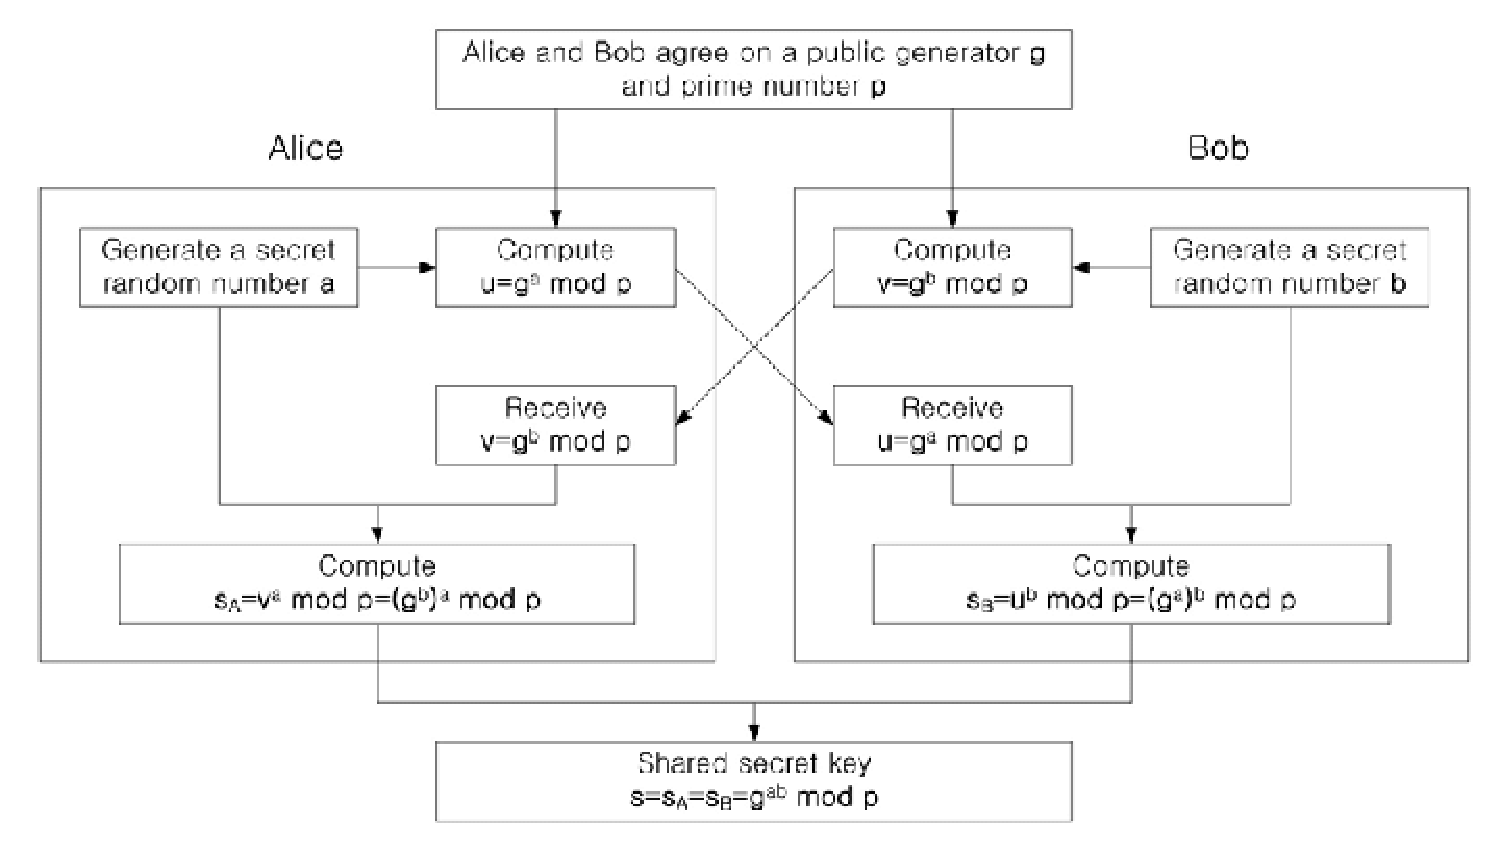
\includegraphics[width=\textwidth]{pictures/diffiehellman.eps}
	\caption{Diffie-Hellman key exchange algorithm\cite{Jeon2014-ag}}
	\label{Diagram, Diffie-Hellman Key Exchange}
\end{figure}
						
Diffie-Hellman key exchange is a way of generating a shared cryptographic key between two participants. The two parties, who are called Alice and Bob, want to generate a shared encryption key to communicate secretly between each other. Alice and Bob first agree on a large prime number \(p\) and a nonzero integer \(g modulo p\). This info is shared between Alice and Bob, and serves as the starting point for the encryption scheme.
						
Next up, Alice picks a secret integer that she keeps to herself, \(a\), 
						
\section{Elliptic Curve Cryptography}
						
\chapter{Peer-to-Peer}
\label{Peer-to-Peer}
Distributed hash tables are a way of pointing content to peers in a distributed network. In addition to indexing content in content-addressed networks like IPFS, they can function as routing tables. A hash table is just a regular key-value store, a mapping from a to b. What makes them distributed is the fact that the data stored is meant to be distributed between peers, with not a single peer keeping all the available data in its DHT, but relaying queries that it can't answer to other peers on the network.
						
\section{Routing}
						
%TODO add more examples of P2P routing
						
\subsection{Distributed Hash Tables}
						
\subsubsection{Kademlia}
Kademlia is a DHT designed by Petar Maymounkov and David Mazières in 2002. It is based on a tree of identifiers which are split across peers on a network.
						
A single query in Kademlia has been shown in real-world tests to result in an average of 3 network hops, meaning that the query gets relayed through two peers before reaching the requested resource.\cite{Roos2013-mb} Network hops are a necessary evil in distributed systems, and Kademlia does well in requiring on average a log(n) queries in a network of n nodes. Since the closeness metric is based on a similarity search rather than a measurement, the closest peer is only closest by the identifier, not by network latency.
						
The randomness of Kademlia is great at averaging the network hops required to reach a scarce resource. The downside is that it also averages everything else, increasing latency to closest connected peers, and increasing the minimum hops to reach a common resource.
